\documentclass[12pt, a4paper]{article}
\usepackage[utf8]{inputenc}
\usepackage{polski}
\usepackage{hyperref}
\usepackage{float}
\usepackage{algorithm}
\usepackage{algpseudocode}
\usepackage{geometry}
\usepackage[table]{xcolor}
\usepackage{graphicx}
\usepackage{subfigure}
\title{\textbf{Optymalna trasa dla kuriera - zastosowanie algorytmu ewolucyjnego}}
\author{Anna Stępień \\ Adam Stelmaszczyk}
\date{\today}
\setlength{\parindent}{0in}
\makeatletter\renewcommand{\ALG@name}{}

\begin{document}
\maketitle

\section{Zadanie}
Celem zadania jest zaprojektowanie algorytmu ewolucyjnego, który zostanie wykorzystany do poszukiwania optymalnej trasy dla kuriera. Zadanie to może być interpretowane jako problem komiwojażera.
Przedstawiona została reprezentacja rozwiązania, metoda sukcesji oraz operatory mutacji i krzyżowania. 
Z punktu widzenia przydatności projektowanego algorytmu, istotne jest przetestowanie go dla różnych parametrów, w szczególności dla:
\begin{itemize}
	\item różnych wartości prawdopodobieństwa mutacji $p_m$ i krzyżowania $p_c$,
	\item różnej liczy miast, które ma odwiedzić kurier $d$.
\end{itemize}

\section{Założenia}
Aplikacja będzie pracować w trybie konsolowym. Na standardowe wejście podawany będzie plik zawierający zestaw współrzędnych geograficznych punktów, które mają zostać odwiedzone przez kuriera. Do obliczenia odległości pomiędzy poszczególnymi punktami zostaną wykorzystane dane pozyskane z \url{http://www.openstreetmap.org/}.
Program będzie wypisywał odpowiedź składającą się z kosztu przejazdu oraz kolejnych miast, które należy odwiedzić na standardowe wyjście.

\subsection{Reprezentacja rozwiązań}

Wierzchołki grafu numerujemy od 0 do $d - 1$. Zakładamy, że $d \in \mathcal{N}$ oraz $d \geq 3$. 
Rozwiązania reprezentujemy jako wektory złożone z $d$ unikalnych liczb. 
Np. $[0,1,2]$ oznacza rozwiązanie złożone z 3 krawędzi: $(0,1), (1,2), (2,0)$. 
W ogólnym przypadku, dla grafu pełnego o $d$ wierzchołkach, liczba unikalnych rozwiązań wynosi $\frac{(d-1)!}{2}$. 
Minimalizowana wartość funkcji celu $f$ to suma wag krawędzi w cyklu dla danego rozwiązania.

\section{Projekt rozwiązania}

\subsection{Schemat algorytmu ewolucyjnego}

\begin{algorithm}[!htb]
\label{ea}
\begin{algorithmic}[1]
\Function{algorytm\_ewolucyjny}{}
  \State $P(0) \gets \{x_1, x_2, \ldots, x_n\}$
  \State $t \gets 0$
  \While{$! stop$}
    \For{$i = 0$ \bf{to} $i = n - 1$}
      \State $a \gets$ selekcja$(P(t))$
      \If{$\mathcal{U}(0, 1) < p_c$}
	\State $b \gets$ selekcja$(P(t))$
	\State $O(t,i) \gets$ mutacja$($krzy{\.z}owanie$(a, b))$
      \Else
	\State $O(t,i) \gets$ mutacja$(a)$
      \EndIf
    \EndFor
    \State $P(t+1) \gets$ sukcesja$(P(t),O(t))$
    \State $t \gets t+1$
  \EndWhile
\EndFunction
\end{algorithmic}
\end{algorithm}

\subsubsection{Mutacja}

Operator mutacji otrzymuje na wejściu prawdopodobieństwo mutacji $p_m$ oraz rozwiązanie długości $d$.
Zwraca rozwiązanie długości $d$, nazywane mutantem.

\begin{enumerate}
 \item Utwórz początkowego mutanta kopiując rozwiązanie wejściowe.
 \item Liczba powtórzeń $R = \lceil d \cdot  p_m \rceil$. Powtórz $R$ razy następujące kroki:
 \item Wylosuj dwa różne indeksy $i, j$ od 0 do $d-1$ zgodnie z rozkładem jednostajnym.
 \item Zamień liczbę na pozycji $i$-tej z liczbą na pozycji $j$-tej w mutancie.
\end{enumerate}

\subsubsection{Krzyżowanie}

Operator krzyżowania na wejściu otrzymuje dwa rozwiązania rodzicielskie długości $d$ i zwraca jedno rozwiązanie potomne długości $d$. 
Jako operator krzyżowania zostanie wykorzystany 
Order1\footnote{\url{http://www.rubicite.com/Tutorials/GeneticAlgorithms/CrossoverOperators/Order1CrossoverOperator.aspx}}:
\begin{enumerate}
 \item Wylosuj dwa indeksy $i, j$ od 0 do $d-1$ zgodnie z rozkładem jednostajnym.
 \item Utwórz jedno puste rozwiązanie potomne długości $d$.
 \item Skopiuj miasta od $i$ do $j$ z pierwszego rodzica do potomka.
 \item Począwszy od lewej strony, wypełnij kolejno puste miejsca potomka tymi miastami drugiego z rodziców, 
których nie ma w skopiowanej sekwencji.
\end{enumerate}

Przykład: \\

Wejściowe rozwiązania rodzicielskie: \\

Rodzic 1
\begin{tabular}{ | c | c | c | c | c | c | c | c |}
  \hline
  2 & 6 &  \cellcolor{green!25}7 & \cellcolor{green!25}1 & \cellcolor{green!25}5 & \cellcolor{green!25}4 & 8 & 3 \\ \hline
\end{tabular}\\
Rodzic 2
\begin{tabular}{ | c | c | c | c | c | c | c | c |}
  \hline
  7 & 5 & 6 & 3 & 8 & 2 & 1 & 4 \\ \hline
\end{tabular}

\begin{enumerate}
 \item Wylosowano $i = 2$, $j = 5$.

 \item Początkowo pusty potomek:
\begin{tabular}{ | c | c | c | c | c | c | c | c |}
 \hline
   &  &  &  &  &  &  &  \\ \hline
\end{tabular}

 \item Skopiowanie sekwencji od $i$ do $j$:
\begin{tabular}{ | c | c | c | c | c | c | c | c |}
 \hline
   &  &  \cellcolor{green!25}7 & \cellcolor{green!25}1 & \cellcolor{green!25}5 & \cellcolor{green!25}4 &  &  \\ \hline
\end{tabular}

 \item Iterujemy przez miasta drugiego rodzica, zaczynamy od 7. 7 już jest w potomku, więc przesuwamy się w prawo.
5 również jest już w potomku, przesuwamy się w prawo. 6 nie ma w potomku, także ją wstawiamy w pierwszym wolnym miejscu
i przesuwamy się w prawo. 3 wstawiamy, 8 i 2 też, 1 i 4 nie. Wyjściowy potomek:

\begin{tabular}{ | c | c | c | c | c | c | c | c |}
 \hline
  6 & 3 &  \cellcolor{green!25}7 & \cellcolor{green!25}1 & \cellcolor{green!25}5 & \cellcolor{green!25}4 & 8 & 2 \\ \hline
\end{tabular}\\

\end{enumerate}

\subsubsection{Selekcja}

Operator selekcji otrzymuje na wejściu populację o rozmiarze $n$. Zwraca jedno losowe rozwiązanie z populacji wejściowej
zgodnie z rozkładem jednostajnym.

\subsubsection{Sukcesja}

Metoda sukcesji na wejściu otrzymuje dwie populacje o rozmiarze $n$: aktualną $P$ oraz populację mutantów $O$.
Wyjściem jest jedna populacja o rozmiarze $n$.

\begin{algorithm}[!htb]
\begin{algorithmic}[1]
\Function{sukcesja}{}
  \For{$i = 0$ \bf{to} $i = n - 1$}
    \If{$f(O(t, i)) < f(P(t, i)) $}
      \State $P(t+1, i) \gets O(t, i)$
    \Else
      \State $P(t+1, i) \gets P(t, i)$
    \EndIf
  \EndFor
\EndFunction
\end{algorithmic}
\end{algorithm}

\subsection{Struktury danych}
	\paragraph{Rozwiązanie}
		Rozwiązanie jest reprezentowane jako tablica $d$ liczb całkowitych, której elementy są numerami miast.
	\paragraph{Populacja}
		Populacja jest reprezentowana jako tablica rozwiązań. Rozmiar populacji jest stały i równy $n = 10d$.

\subsection{Założenia programu}
\begin{description}
	\item[Wejście] \hfill \\
Wejściem dla algorytmu jest plik tekstowy zawierający w kolejnych liniach współrzędne geograficzne miejsc, które ma odwiedzić kurier. 
$
52.259 21.020 \\ 
50.060 19.959 \\
54.360 18.639 \\
52.399 16.900 \\
53.120 18.010 \\
51.110 17.030 \\
51.770 19.459 \\
$
	\item[Wyjście] \hfill \\
	Wyjściem algorytmu jest plik tekstowy zawierający koszt najtańszego cyklu znalezionego przez algorytm oraz współrzędne kolejnych miast, które należy odwiedzić.
	\item[Kryteria stopu] \hfill \\
	Warunkiem zatrzymania algorytmu jest wywołanie $10^5d$ razy funkcji oceny, gdzie $d$ to rozmiar problemu (liczba miast).
	\item[Parametry] \hfill \\
	Na wejście programu możliwe jest podanie dwóch parametrów określających odpowiednio:
		\begin{itemize}
			\item prawdopodobieństwo mutacji $p_m$ (domyślna wartość 0,9)
			\item prawdopodobieństwo krzyżowania $p_c$ (domyślna wartość 0,1)
		\end{itemize}
		W przypadku, gdy parametry te nie zostaną sprecyzowane, stosowane są wartości domyślne.
		\item Obliczanie odległości pomiędzy miastami
		Do obliczenia odległości pomiędzy punktami na trasie kuriera zostaną wykorzystane dane pozyskane z~OpenStreetMap oraz biblioteka graphhopper\footnote{\url{http://graphhopper.com}}.

\end{description}

\section{Testy algorytmu ewolucyjnego}
Początkowo działanie algorytmu ewolucyjnego zostało zweryfikowane na zestawie danych, dla których znane były rozwiązania optymalne. W tym celu aplikacja została dostosowana do obsługi drugiego formatu danych wejściowych - macierzy zawierającej koszty połączeń pomiędzy poszczególnymi miastami.
Działanie algorytmu zostało zbadane dla następujących parametrów:
\begin{itemize}
	\item prawdopodobieństwa mutacji $p_m$,
	\item prawdopodobieństwa krzyżowania $p_c$,
	\item liczby miast.
\end{itemize}

Podczas testowania analizowane były następujące kombinacje wartości wartości prawdopodobieństwa mutacji $p_m$ i prawdopodobieństwa krzyżowania $p_c$.

\bigskip

Dla ustalonej wartości $p_c = 0,9$ - zbadanie wpływu zmian $p_m$:
\begin{center}
\begin{tabular}{|l|l|l|l|}
\hline
\multicolumn{4}{|c|}{$(p_m; p_c)$} \\
\hline
(0,1; 0,9) & (0,5; 0,9) & (0,9; 0,9) & (1; 0,9)\\
\hline
\end{tabular}
\end{center}

\bigskip

Dla wyłączonego krzyżowania $p_c = 0$ - zbadanie wpływu zmian $p_m$:
\begin{center}
\begin{tabular}{|l|l|l|l|}
\hline
\multicolumn{4}{|c|}{$(p_m; p_c)$} \\
\hline
(0,1; 0) & (0,5; 0) & (0,9; 0) & (1; 0)\\
\hline
\end{tabular}
\end{center}

\bigskip

Dla ustalonej wartości $p_m = 0,1$ - zbadanie wpływu zmian $p_c$:
\begin{center}
\begin{tabular}{|l|l|l|l|}
\hline
\multicolumn{4}{|c|}{$(p_m; p_c)$} \\
\hline
(0,1; 0,1) & (0,1; 0,5) & (0,1; 0,9) & (0,1; 1)\\
\hline
\end{tabular}
\end{center}

\bigskip

Dla wyłączonej mutacji $p_m = 0$ - zbadanie wpływu zmian $p_c$:
\begin{center}
\begin{tabular}{|l|l|l|l|}
\hline
\multicolumn{4}{|c|}{$(p_m; p_c)$} \\
\hline
(0; 0,1) & (0; 0,5) & (0; 0,9) & (0; 1)\\
\hline
\end{tabular}
\end{center}

\bigskip

Pojedynczy przypadek testowy polegał na uruchomieniu algorytmu ewolucyjnego dla określonego 
problemu i zadanych wartości prawdopodobieństwa mutacji $p_m$ i prawdopodobieństwa 
krzyżowania $p_c$. Każdy przypadek testowy uruchomiony był niezależnie $RUNS = 15$ razy.\\
\\
Poszczególne przypadki testowe uruchamiano dla ustalonej wartości ziarna generatora 
liczb pseudolosowych -- w ten sposób sekwencje liczb pseudolosowych dla każdej wersji 
algorytmu były jednakowe, co umożliwi porównanie ich skuteczności.\\
\\
W~celu porównania skuteczności poszczególnych ustawień algorytmu, dla każdego z~przypadków testowych zostały wykreślone 
dystrybuanty empiryczne -- miarą jakości algorytmu jest różnica pomiędzy optymalnym 
kosztem cyklu a~kosztem obliczonym przez algorytm.

\begin{table}[h]
  \centering
  \begin{tabular}{ | c | c | }
    \hline
    Liczba miast & Minimum\\
    \hline
    17 & 2085\\
    \hline
    26 & 937\\
    \hline
    42 & 699\\
    \hline
    48 & 10628\\
    \hline
  \end{tabular}
  \caption{Długość optymalnych cykli}
\end{table}

\section{Wyniki testów}

\subsection{Wpływ prawdopodobieństwa mutacji}
\begin{figure}[H]
\centering
\mbox{\subfigure[$p_c = 0,9$]{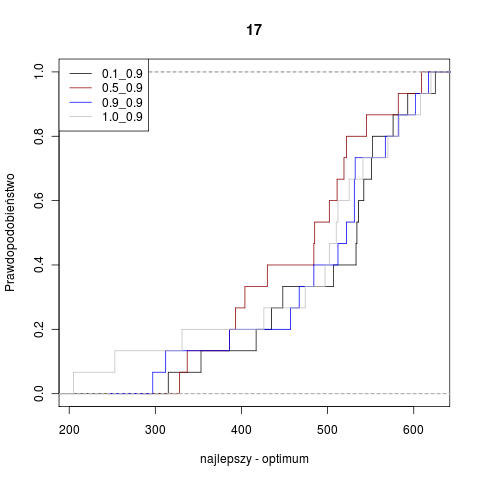
\includegraphics[width=.5\textwidth]{../tests/old/17m.png} }\quad
\subfigure[$p_c = 0$]{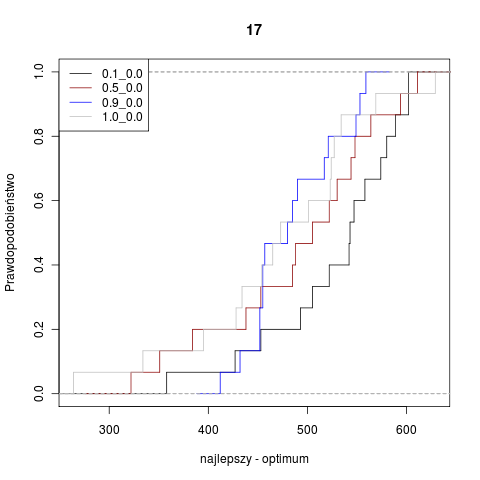
\includegraphics[width=.5\textwidth]{../tests/normal/17m.png} } 
}
\caption{Wpływ mutacji na działanie algorytmu - 17 miast}
\end{figure}

\begin{figure}[H]
\centering
\mbox{\subfigure[$p_c = 0,9$]{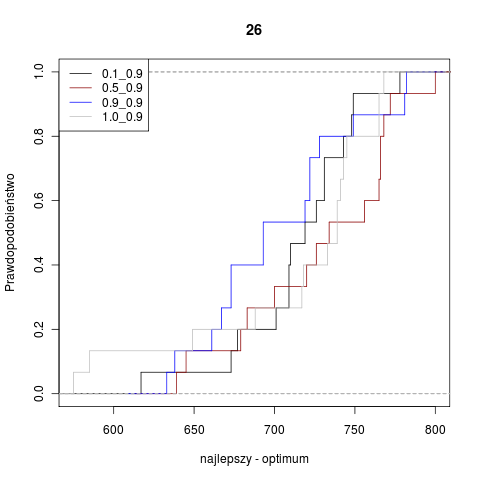
\includegraphics[width=.5\textwidth]{../tests/old/26m.png} }\quad
\subfigure[$p_c = 0$]{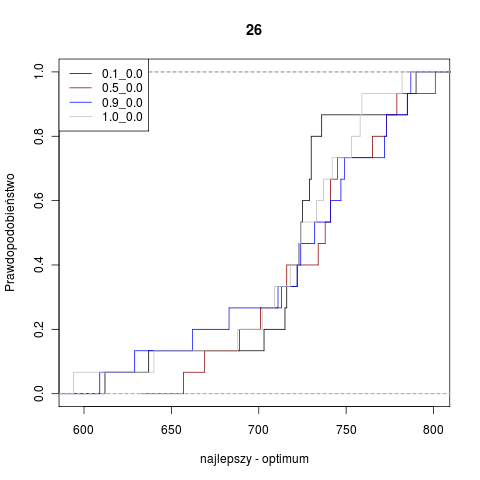
\includegraphics[width=.5\textwidth]{../tests/normal/26m.png} } 
}
\caption{Wpływ mutacji na działanie algorytmu - 26 miast}
\end{figure}

\begin{figure}[H]
\centering
\mbox{\subfigure[$p_c = 0,9$]{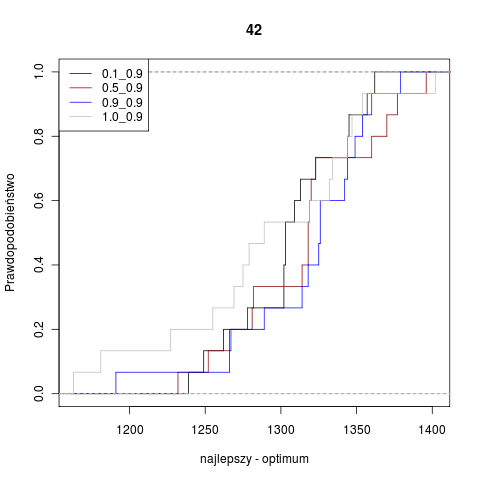
\includegraphics[width=.5\textwidth]{../tests/old/42m.png} }\quad
\subfigure[$p_c = 0$]{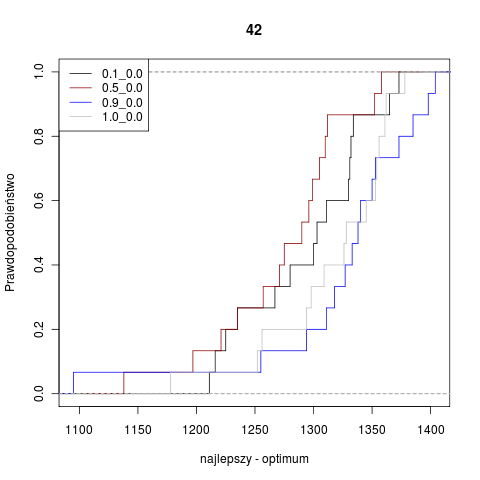
\includegraphics[width=.5\textwidth]{../tests/normal/42m.png} } 
}
\caption{Wpływ mutacji na działanie algorytmu - 42 miasta}
\end{figure}

\begin{figure}[H]
\centering
\mbox{\subfigure[$p_c = 0,9$]{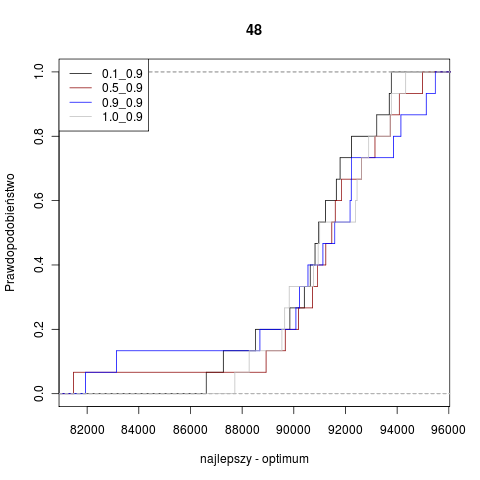
\includegraphics[width=.5\textwidth]{../tests/old/48m.png} }\quad
\subfigure[$p_c = 0$]{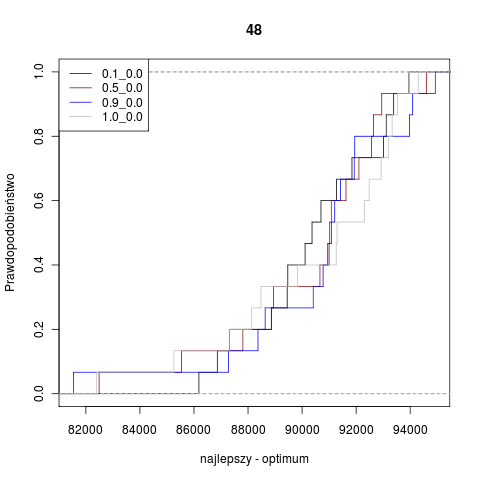
\includegraphics[width=.5\textwidth]{../tests/normal/48m.png} } 
}
\caption{Wpływ mutacji na działanie algorytmu - 48 miast}
\end{figure}

\subsection{Wpływ prawdopodobieństwa krzyżowania}
\begin{figure}[H]
\centering
\mbox{\subfigure[$p_m = 0,1$]{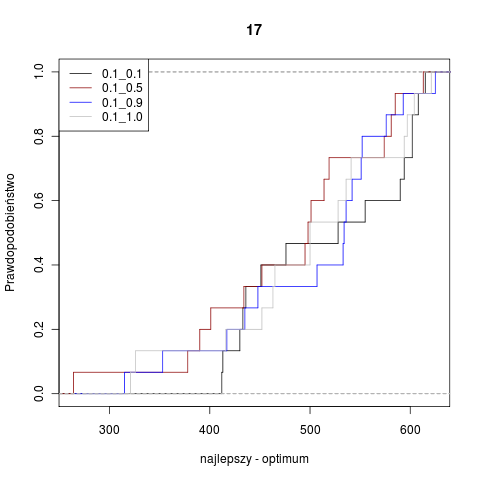
\includegraphics[width=.5\textwidth]{../tests/old/17c.png} }\quad
\subfigure[$p_m = 0$]{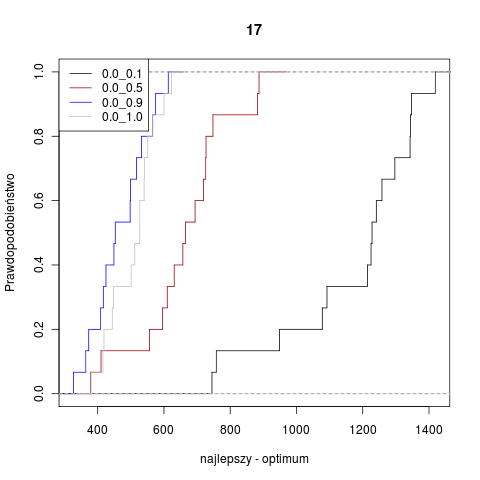
\includegraphics[width=.5\textwidth]{../tests/normal/17c.png} } 
}
\caption{Wpływ krzyżowania na działanie algorytmu - 17 miast}
\end{figure}

\begin{figure}[H]
\centering
\mbox{\subfigure[$p_m = 0,1$]{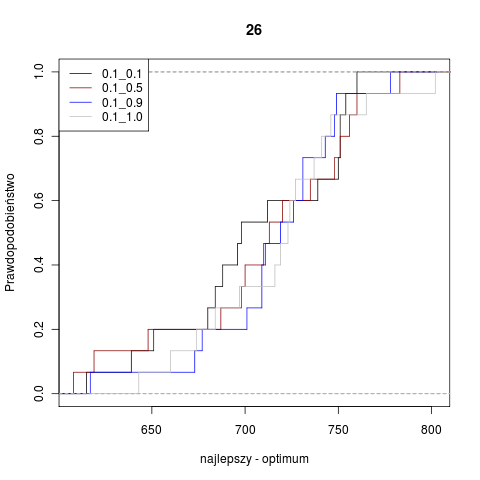
\includegraphics[width=.5\textwidth]{../tests/old/26c.png} }\quad
\subfigure[$p_m = 0$]{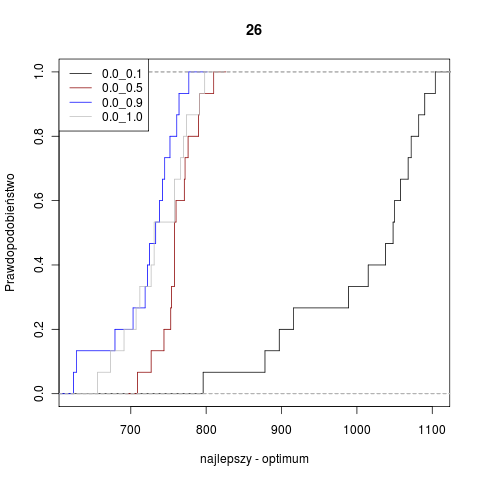
\includegraphics[width=.5\textwidth]{../tests/normal/26c.png} } 
}
\caption{Wpływ krzyżowania na działanie algorytmu - 26 miast}
\end{figure}

\begin{figure}[H]
\centering
\mbox{\subfigure[$p_m = 0,1$]{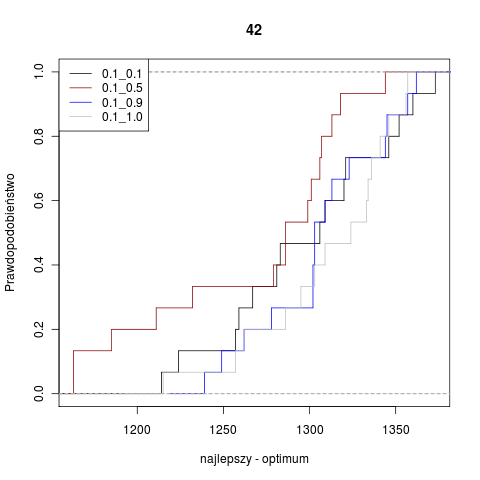
\includegraphics[width=.5\textwidth]{../tests/old/42c.png} }\quad
\subfigure[$p_m = 0$]{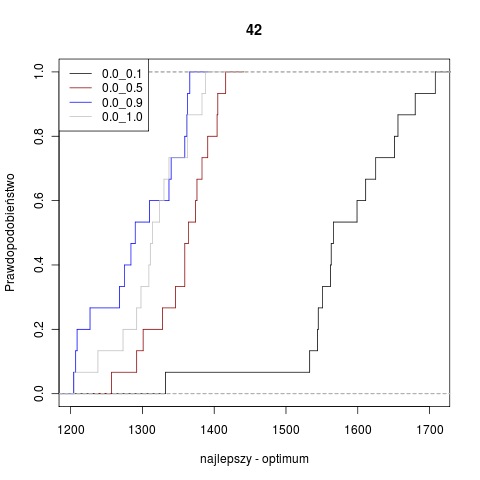
\includegraphics[width=.5\textwidth]{../tests/normal/42c.png} } 
}
\caption{Wpływ krzyżowania na działanie algorytmu - 42 miasta}
\end{figure}

\begin{figure}[H]
\centering
\mbox{\subfigure[$p_m = 0,1$]{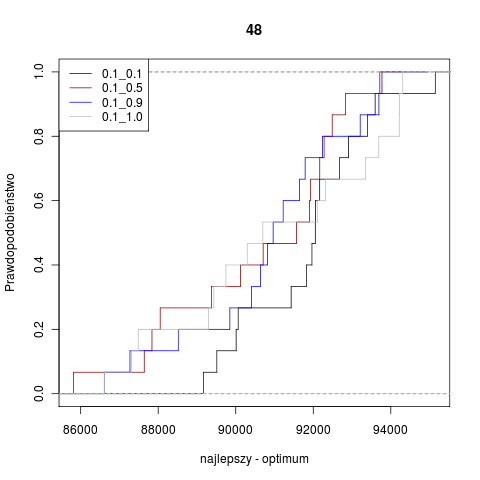
\includegraphics[width=.5\textwidth]{../tests/old/48c.png} }\quad
\subfigure[$p_m = 0$]{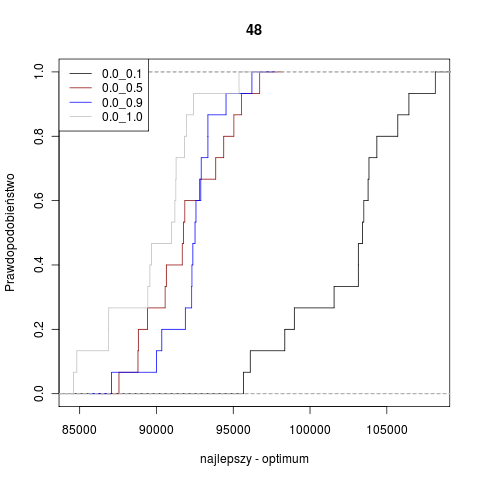
\includegraphics[width=.5\textwidth]{../tests/normal/48c.png} } 
}
\caption{Wpływ krzyżowania na działanie algorytmu - 48 miast}
\end{figure}

\subsection{Porównanie z algorytmem zachłannym}

Algorytm zachłanny zaczyna od losowego miasta. Następnie przechodzi do najbliższego 
nieodwiedzonego miasta. Kończy działanie w momencie odwiedzenia wszystkich miast, czyli
znalezienia cyklu. Jak na szybkość i prostotę algorytmu, znajdowane rozwiązanie są zaskakująco 
dobre, znacznie lepsze niż te otrzymywane przez którykolwiek algorytm ewolucyjny.

\begin{table}[h]
\centering
	\begin{tabular}{ | c | c | c | c | } 
		\hline
  		Liczba miast & Optimum & Algorytm zachłanny & Algorytm ewolucyjny \\
  		\hline
  		17 & 2085 & 2178 & 2349 \\
  		\hline
  		26 & 937 & 965 & 1522\\
  		\hline
  		42 & 699 & 864 & 1794\\
  		\hline
  		48 & 10628 & 37928 & 92101\\
  		\hline
	\end{tabular}
\caption{Najlepsze wyniki uzyskane przez algorytm zachłanny oraz ewolucyjny.}
\end{table}

\subsection{Testy dla danych pochodzących z OpenStreetMap}
Na potrzeby testów aplikacji wykorzystaliśmy dane OpenSteetMap dla obszaru Polski dostępne na stronie\footnote{{http://download.geofabrik.de/europe/poland.html}}. Dane te zostały przetworzone za pomocą biblioteki graphhopper, a następnie wykorzystane do obliczania odległości drogowych pomiędzy zadanymi punktami/miastami. 

\subsection{Czas wykonania dla grafów losowych}

Przebadano czas wykonania na grafach losowych o 5, 10, 20 oraz 40 miastach.
Dla każdej liczby miast brano pod uwagę uśredniony czas z 10 prób (na różnych grafach losowych).
Badanym algorytmem był algorytm ewolucyjny z $p_m=0,1$ oraz $p_c=0,9$.
Losowy graf o $d$ miastach generowano w następujący sposób:

\begin{enumerate}
 \item Pobierz $d$ losowych położeń miast Polski.
 \item Na podstawie ich położeń wygeneruj wejściową macierz odległości.
\end{enumerate}

Wyniki eksperymentów przedstawiono w poniższej tabeli:

\begin{table}[h]
\centering
	\begin{tabular}{ | c | c | c | c | } 
		\hline
  		Liczba miast & Średni czas [s] \\
  		\hline
  		5 & 8,3 \\
  		\hline
  		10 & 18,2 \\
  		\hline
  		20 & 91,9 \\
  		\hline
  		40 & 319,2 \\
  		\hline
	\end{tabular}
\caption{Średnie czasy wykonania uzyskane przez algorytm ewolucyjny.}
\end{table}

Na poniższym grafie zaznaczono czerwonymi punktami punkty pomiarowe:

\begin{figure}[H]
\centering
  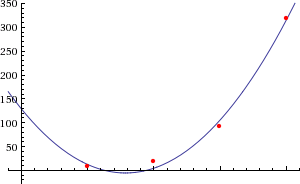
\includegraphics[width=.5\textwidth]{time.png}
\end{figure}

Niebieska linia przedstawia funkcję $54,25x^2 - 170,55x + 128,75$ aproksymującą
złożoność czasową testowanego algorytmu ewolucyjnego. Funkcja ta została znaleziona przy pomocy
\url{http://www.wolframalpha.com}. Podwojenie wielkości danych wejściowych $d$ (liczby miast) powoduje
kwadratowy przyrost długości obliczeń, stąd złożoność obliczeniowa 
testowanego algorytmu to O$(d^2)$.

\section{Wnioski}
%TODO odpowiednio zmodyfikować wnioski
Na podstawie otrzymanych wyników można zauważyć, że niezależnie od przyjętych wartości 
prawdopodobieństwa krzyżowania i~mutacji algorytm ewolucyjny nigdy nie osiągnął optimum.
 Wraz ze wzrostem rozmiaru problemu, otrzymywane wyniki były coraz bardziej odległe od 
poszukiwanego optimum -- w~przypadku 48 miast zauważalne jest znaczące pogorszenie w~stosunku 
do wyników otrzymywanych dla problemów o~mniejszym rozmiarze tj. 17, 26, czy 42.\\
\\
Analiza wpływu wartości prawdopodobieństwa mutacji i~krzyżowania pozwala stwierdzić, 
że większy wpływ na działanie algorytmu ewolucyjnego dla problemu komiwojażera miała mutacja. 
Całkowite wyłącznie mutacji wyraźnie pogarsza jakość otrzymywanych wyników. 
Sama jej obecność (nawet z~niewielkim prawdopodobieństwem) wyraźnie wpływa na poprawę 
otrzymywanych wyników. Ma to swoje uzasadnienie praktyczne - mając dowolny cykl, łatwo
jest go poprawić dokonując małych zmian.\\
\\
Zaimplementowany operator krzyżowania Order1, nie wpłynął w~znacznym 
stopniu na jakość otrzymywanych rozwiązać. Spowodowane jest to tym, że
operator krzyżowania wprowadza ogromne zmiany do rozwiązania, praktycznie rozrywając dwa cykle, 
więc istnieje bardzo mała szansa poprawy. Niemniej obecność operatora krzyżowania jest wskazana, 
a~wartość prawdopodobieństwa krzyżowania powinna przyjmować dosyć dużą wartość.\\
\\
W~porównaniu do algorytmu zachłannego, algorytm ewolucyjny zdecydowanie gorzej poradził sobie 
z~problemem komiwojażera. Warto zatem do populacji początkowej dla algorytmu ewolucyjnego
wprowadzać po kilka różnych rozwiązań wygenerowanych przez algorytm zachłanny. Gwarantuje to znacznie lepszy
start, bliżej optimum globalnego. 

\nocite{*}
\bibliographystyle{plain}
\bibliography{references}
\end{document}
